\section{Ejercicio 3}

\subsection{Introducción}
\noindent El problema presentado nos pide encontrar el MCS entre un cografo al que llamaremos $'G'$ (con $\#G$ vértices) y un grafo completo $k_n$ (de $n$ vértices).\\
Para resolver este problema observamos que si el cografo $G$ tiene menor o igual cantidad de vértices que el completo $k_n$ , osea si $\#G \leq n$, el subgrafo común de mayor cantidad de aristas sera  G, pues seguro existe contenido en el completo uno isomorfo a G ya que cada nodo de G lo puedo asignar(en la función isomorfismo $'f'$) a un vértice del completo (porque son menos) y es inmediato ver que en si dos vértices $v_1$,$v_2$ tenían una arista que los unía en G tendrán una una vez aplicado el isomorfismo (habrá arista de $f(v_1)$ a $f(v_2)$) pues es un completo y están todas las aristas posibles.\\
El problema entonces estará en el caso en el que $\#G > n$, es en este caso que observamos que el problema es equivalente a:\\
\emph{'Encontrar el subgrafo $g_n$ de $G$ de $n$ nodos con la mayor cantidad de aristas posibles'}, pues cualquier subgrafo de $G$ de $n$ nodos es isomorfo a un subgrafo de $k_n$, y podemos garantizar que se maximizan las cantidad de aristas como pide el problema ya que si $g_n$ es el grafo de n nodos de mayor cantidad de aristas, no puede haber uno con menos nodos y mas aristas (de haberlo digamos $g_{<n}$ podríamos agregarle $k$ nodos cualesquiera hasta llegar a n, $g_{<n+k}$, y resultaría $cantAristas(g_{<n+k})>cantAristas(g_n)$, contradiciendo la hipótesis de ser $g_n$ el de mayor aristas de $n$ vértices) ni tampoco serviría un subgrafo con mas nodos pues ya dejaría de ser subgrafo de $K_n$.\\
Este último problema entonces es el que intentaremos resolver. Para poder realizarlo en tiempo polinomial aprovecharemos la característica de $G$ de ser cografo.

\subsection{Desarrollo}

\noindent Para resolver este problema entenderemos a los cografos mediante la definición alternativa de cografo, esta es que: los cografos son $K_1$, la unión disjunta de cografos y el 'join' entre 2 cografos (aristas entre todos los nodos de un cografo y todos los nodos del otro).
\subsubsection{Implementación}
La implementación de este algoritmo se divide en 2 grandes etapas:
\begin{enumerate}
\item Creación del cotree:\\
 Un cotree es un árbol enraizado asociado a un cografo. Todo cografo puede representarse univoca mente con un cotree (hay mas de un cotree que representa un mismo cografo pero un cotree determina un único cografo,excepto isomorfismos).\\
 La estructura de cotree es una serie de nodos en forma de árbol en el que cada nodo tiene un id particular. El id de las hojas es un identificador de cada nodo del cografo, mientras que el id de los nodos interiores determina si sus subárboles hijos deben ser unidos disjuntamente o en 'join'.\\
Para armar el cotree el algoritmo será:
\begin{itemize}
\item Si el grafo de entrada es un $k_1$ crear una hoja con el id correspondiente al vértice.
\item Identificar si hay mas de una componente conexa, de haberlas, crear un nodo con el id='Unión' y llamar recursivamente al algoritmo en cada componente conexa y anexar los resultados de cada subproblema como hijos de ese nodo 'Unión'.
\item Si hay una única componente conexa crear un nodo de 'Join' y los hijos serán la llamadas recursivas con el complemento de cada componente conexa del complemento del grafo de entrada.
\end{itemize}
Una vez realizado esto tendremos un cotree válido del cografo.\\
Para simplificar la programación del siguiente inciso procedemos a binarizar el cotree, es decir, expresarlo en un árbol binario. Esto puede hacerse ya que es indistinto para la interpretación del cotree si se unen disjuntamente $x$ cantidad de cografos como una operación atómica o como una sucesión de operaciones binarias; el resultado es el mismo cografo. Lo mismo sucede con el 'join': si quisiéramos hacer un join entre 3 o mas cografos, el resultado sería el mismo al hacer todos los joins juntos que ir tomando de a pares e ir haciendo el join entre esos pares.\\
Para implementar esta binarización recorremos el cotree y para aquellos nodos internos $u$ que tengan mas de 2 hijos, le dejamos uno de esos hijos, $w$, y le ponemos como segundo hijo un nodo del mismo tipo que $u$ (Join o Unión, ya que todos los nodos internos del cotree son, o bien join, o bien unión), llamémoslo $v$. Como hijos de $v$ ponemos a los hijos restantes de $u$ (que son todos los hijos de $u$ menos el nodo $w$). Luego de hacer esa corrección, procedemos a llamar recursivamente a los dos hijos de $u$ ($w$ y $v$).
\item Comparar alternativas:
\begin{itemize}
\item En esta etapa lo que se hará será, dado el cotree $'T'$(binario) asociado al cografo y un entero $n$ (cantidad de vértices del completo), resolveremos el problema de encontrar el subgrafo(del cografo) de $n$ nodos con la mayor cantidad posible de aristas aplicando el siguiente algoritmo(la función 'solución(..)'):\\
tomamos la raíz del cotree $T$ y comparamos todas las posibilidades de tomar n nodos de los sub-cotrees (sus hijos izq y der) para esto llamamos recursivamente a la función iterando(sobre 'i' de 0 a n) la cantidad de vértices a tomar de cada sub-cotree (solución(izq,i) y solución(de,n-i)) y entonces la cantidad de aristas en la solución optima sera una de las siguientes opciones:
  \item la suma de las del izq y der que resultaron ser la combinación máxima, en caso de la raíz ser una 'Unión'.
  \item la suma de las de izq y der que resultaron ser la combinación máxima una vez que a dicha combinación le sumamos el producto de la cantidad de vértices en izq por la cantidad de vértices en der, en caso de ser 'Join'.
 \item 0 aristas tendrá una hoja (un vértice).
 Los nodos pertenecientes a esta solución optima son entonces los cuales se usan en la combinación máxima.
\end{itemize}
Basta entonces llamar a la función solución pasando por parámetro el cotree binario previamente creado y  el tamaño (cantidad de vértices) del completo, para que el algoritmo devuelva los nodos que forman en subgrafo con mayor cantidad de aristas de n nodos.\\
Restaría sólo mostrar el resultado.

\end{enumerate}

\subsubsection{Correctitud}
Para verificar la correctitud de este algoritmo analizaremos 2 incisos.
\begin{enumerate}
\item El subgrafo retornado es un subgrafo(o isomorfo a un subgrafo) tanto del cografo ($G$) como del completo ($K_n$).
\item El subgrafo retornado es optimo (tiene la mayor cantidad de aristas que un subgrafo de ambos puede tener).\\
\\
El inciso 1. es casi inmediato, pues por como se arma el grafo, siempre trabajando sobre subgrafos de $G$, se confirma que el grafo retornado ($'sol'$) es subgrafo de G y como tiene máximo n nodos (tiene exactamente n cuando $\#V(G) > n$ y tiene $\#V(G)$ cuando $n \geq \#V(G)$) tiene que ser subgrafo de $k_n$ pues todo grafo de menos (o igual a n) de n nodos es subgrafo del completo de n nodos ya que si arbitrariamente asignas cada nodo del dicho grafo a cualquiera del completo, todas las aristas del grafo estarán en el completo, por lo tanto concluimos que la solución también es subgrafo de $K_n$.\\ \\
El inciso 2. requiere de un mayor análisis: es óptimo el subgrafo retornado pues las operaciones de Join y de Unión es equivalente hacerlas entre muchas componentes a la vez que hacerlas de a pares como ya explicamos mas arriba en la subsección ``Algoritmo''.\\
Además, dados 2 cografos $C_1$ y $C_2$, subgrafos de $C$ cografo, entrelazados por una Unión o un Join digamos $C:= C_1 \bigtriangleup C_2$ donde $\bigtriangleup$ es operador de Unión o de Join indistintamente.\\
El subgrafo de $C$ de mayor cantidad de aristas de $n_i$ vértices, sera algún $c_1'$ subgrafo de $C_1$ $\bigtriangleup$ algún $c_2'$ subgrafo de $C_2$, pues es evidente que los vértices de éste subgrafo máximo tiene que estar en $C_1$ o en $C_2$ (ya que allí están todos los vértices posibles) y también podemos afirmar que de haber aristas entre $C_1$ y $C_2$ es debido a que $\bigtriangleup$ es un Join (pues si era Unión no habría arista alguna que cruce de $C_1$ a $C_2$) y por lo tanto en ambos casos el subgrafo de $C$ de $n_i$ nodos que maximiza la cantidad de aristas es de la forma:
$c_1' \bigtriangleup c_2'$ con $c_1',c_2'$ subgrafos de sus correspondientes $C_j$  con j=1,2.\\
Como el algoritmo aplica recursivamente este proceso de seleccionar el mejor par $(c_1',c_2')$ (como está descripto mas arriba) probando todos los posibles tamaños de éstos y pidiendo recursivamente los óptimos de subcografos mas chicos. se garantiza que cada paso de selección es optimo y por lo tanto la selección global, con todo el cografo G también lo es. 

\end{enumerate}

\subsection{Complejidad}
La complejidad del algoritmo la vamos a calcular mirando el pseudocódigo del mismo.
Como dijimos anteriormente, el algoritmo se divide en dos grandes etapas:
\begin{itemize}
	\item Creación del cotree
    \item Comparar alternativas
\end{itemize}
\subsubsection*{Creación del cotree}\;
La creación del cotree se divide en dos partes: primero se genera un cotree m-ario, y luego se lo binariza para que el cotree quede binario.
Veamos el pseudocógido de la generación del cotree m-ario: \\
\small{}
\begin{algoritmo}{$make\_cotree$}{$vector<Vertice>* g, Cotree* root$}{}
	\If(\hfill {$\triangleright$ $\mathcal{O}$($N$)}){$obtener\_nodos\_posta($g$) == 1$} {
    	$root->id$ $\gets$ dame\_unico\_nodo($g$) \com*{$\mathcal{O}$($N$)}
        $root->hijos$ $\gets$ $vector<Cotree*>$() \com*{$\mathcal{O}$(1)}
        $root->nodos$.push\_back($root->id$) \com*{$\mathcal{O}$(1)}
        \tipo{return} \com*{$\mathcal{O}$(1)}
    } \Else {
    	$vector<vector<Vertice> >$ componentes $\gets$ separar\_componentes\_conexas($g$) \com*{$\mathcal{O}$($N^2$)}
        \tipo{int} $cc \gets componentes$.size() \com*{$\mathcal{O}$(1)}
        \If(\hfill {$\triangleright$ $\mathcal{O}$(1)}){$cc == 1$} {
        	$root->id \gets$ -1 \com*{$\mathcal{O}$(1)}
            $vector<Vertice> auxx \gets$ complementar(componentes[0]) \com*{$\mathcal{O}$($N^2$)}
            $vector<vector<Vertice> > componentes\_complementadas \gets$ separar\_componentes\_conexas(\&auxx) \com*{$\mathcal{O}$($N^2$)}
            \If(\hfill {$\triangleright$ $\mathcal{O}$(1)}){$componentes\_complementadas.size() != 1$} {
            	\For(\hfill {$\triangleright$ $\mathcal{O}$($N$)}){($i$ = 0; $i < componentes\_complementadas.size()$; $i$++)}{
					Cotree* co\_aux $\gets$ new Cotree() \com*{$\mathcal{O}$(1)}
                    $vector<Vertice> grafo\_aux \gets$ complementar(componentes\_complementadas[$i$]) \com*{$\mathcal{O}$($N^2$)}
                    make\_cotree(\&grafo\_aux, co\_aux) \com*{$\mathcal{O}$(1)}
                    \tipo{iterator} $inicio \gets co\_aux->nodos$.begin() \com*{$\mathcal{O}$(1)}
          			\tipo{iterator} $fin \gets co\_aux->nodos$.end() \com*{$\mathcal{O}$(1)}
                    \While(\hfill {$\triangleright$ $\mathcal{O}$($N$)}){inicio != fin} {
                      $root->nodos.push\_back$(*inicio) \com*{$\mathcal{O}$(1)}
                      inicio++ \com*{$\mathcal{O}$(1)}
                    }
                    $root->hijos.push\_back$(co\_aux) \com*{$\mathcal{O}$(1)}
				}
                \tipo{return} \com*{$\mathcal{O}$(1)}
            }
        } \Else {
        	$root->id \gets$ -2 \com*{$\mathcal{O}$(1)}
            \For(\hfill {$\triangleright$ $\mathcal{O}$($N$)}){$i$ = 0; $i <$ cc; $i$++} {
            	$Cotree* co\_aux \gets$ new Cotree() \com*{$\mathcal{O}$(1)}
                make\_cotree(\&componentes[i], co\_aux) \com*{$\mathcal{O}$(1)}
                \tipo{iterator} $inicio \gets co\_aux->nodos$.begin() \com*{$\mathcal{O}$(1)}
          		\tipo{iterator} $fin \gets co\_aux->nodos$.end() \com*{$\mathcal{O}$(1)}
                \While(\hfill {$\triangleright$ $\mathcal{O}$($N$)}){inicio != fin} {
                  $root->nodos$.push\_back(*inicio) \com*{$\mathcal{O}$(1)}
                  inicio++ \com*{$\mathcal{O}$(1)}
                }
                $root->hijos.push\_back(co\_aux)$ \com*{$\mathcal{O}$(1)}
            }
            \tipo{return} \com*{$\mathcal{O}$(1)}
        }
    }
\end{algoritmo}
\normalsize{}
Esta función usa algunas funciones auxiliares, como $obtener\_nodos\_posta$ que recorre todos los $N$ nodos del cografo, y cuenta la cantidad de nodos que tienen en $true$ el campo $pertenece$, o sea, cuenta la cantidad de nodos que realmente tiene el cografo (si algún nodo tiene el campo $pertenece$ en $false$, ése grafo es un subgrafo del cografo original). Esa función tiene complejidad $\mathcal{O}(N)$ ya que recorre los $N$ nodos y en cada iteración hace pasos constantes (preguntar el valor de $pertenece$ y sumar uno al contador de nodos).\\
Otra función que usa el algoritmo es $dame\_unico\_nodo$ la cual recorre todo el subgrafo del cografo original buscando el único nodo que pertenece a ése subgrafo. También cuenta con complejidad $\mathcal{O}(N)$ ya que recorre todos los nodos del subgrafo y realiza operaciones constantes en cada iteración. \\
Por último, hay otras dos funciones que ejecuta el algoritmo:
\begin{itemize}
	\item $separar\_componentes\_conexas$: separa el grafo en las distintas componentes conexas. Cada componente conexa tiene los $N$ nodos del grafo original, pero sólo sus propios nodos tendrán $true$ en el campo $pertenece$; los demás tendrán $false$.
    \item $complementar$: complementa el grafo pasado por parámetro. Lo hace en $\mathcal{O}(N^2)$ ya que para cada nodo, recorre su lista de adyacencia fijándose qué nodos no están en la lista para agregarlos en la lista de adyacencia correspondiente al mismo nodo en el grafo complemento.
\end{itemize}
En el peor caso (si hubo un Join), en cada iteración se complementa el grafo, que cuesta $\mathcal{O}(N^2)$, y luego se complementa cada componente conexa para llamar recursivamente. En total, entonces tenemos que la complejidad es $\mathcal{O}(N)$*$\mathcal{O}(N^2)$ = $\mathcal{O}(N^3)$, siendo $N$ la cantidad de nodos del cografo. \\ 

Veamos ahora la complejidad de binarizar el cotree: \\
\begin{algoritmo}{$binarizar$}{$Cotree* src$}{}
	\If(\hfill {$\triangleright$ $\mathcal{O}$(1)}){$src->hijos.size() > 2$} {
    	$Cotree* aux \gets$ new Cotree() \com*{$\mathcal{O}$(1)}
    	$aux->id \gets src->id$ \com*{$\mathcal{O}$(1)}
        \For(\hfill {$\triangleright$ $\mathcal{O}$($N'$)}){$i = src->hijos$.size()-1; $i >$ 0; i--} {
        	$aux->hijos$.push\_back($src->hijos$[i]) \com*{$\mathcal{O}$(1)}
            \tipo{iterator} inicio $\gets src->hijos[i]->nodos$.begin() \com*{$\mathcal{O}$(1)}
            \tipo{iterator} fin $\gets src->hijos[i]->nodos$.end() \com*{$\mathcal{O}$(1)}
            \While(\hfill {$\triangleright$ $\mathcal{O}$($N'$)}){inicio != fin} {
              $aux->nodos.push\_back$(*inicio) \com*{$\mathcal{O}$(1)}
              inicio++ \com*{$\mathcal{O}$(1)}
            }
            $src->hijos.pop\_back$() \com*{$\mathcal{O}$(1)}
        }
        $src->hijos$.push\_back(aux) \com*{$\mathcal{O}$(1)}
        binarizar($src->hijos$[0]) \com*{$\mathcal{O}$(1)}
        binarizar($src->hijos$[1]) \com*{$\mathcal{O}$(1)}
    } \Else {
    	\If(\hfill {$\triangleright$ $\mathcal{O}$(1)}){$src->hijos.size() == 2$}{
        	binarizar($src->hijos$[0]) \com*{$\mathcal{O}$(1)}
    		binarizar($src->hijos$[1]) \com*{$\mathcal{O}$(1)}
        } \Else {
        	\If(\hfill {$\triangleright$ $\mathcal{O}$(1)}){$src->hijos.size() == 1$} {
            	binarizar($src->hijos$[0]) \com*{$\mathcal{O}$(1)}
            }
        }
    }
\end{algoritmo}
Sea $N'$ la cantidad de nodos del cotree y $N$ la cantidad de nodos del cografo. Notemos que la función binarizar se va invocando recursivamente por cada nodo del cotree, y si en cada llamada realiza $\mathcal{O}$($N'$) operaciones, en total la función binarizar tiene complejidad $N'$*$\mathcal{O}$($N'$) = $\mathcal{O}$($N'^2$), siendo $N'$ la cantidad de nodos del cotree. Pero como $N' \in \mathcal{O}($N$)$ (ya que si el cotree tiene $N$ hojas, por ser un árbol exactamente binario, tiene $N-1$ nodos internos, entonces la cantidad de nodos del cotree es $N$+$N$-1 = 2$N$-1 = $N'$; notar también que las hojas del cotree corresponden a los nodos del cografo), entonces queda que la complejidad de binarizar es $\mathcal{O}$($N^2$), siendo $N$ la cantidad de nodos del cografo. \\

Por último, tenemos que calcular la complejidad del algoritmo que compara las distintas alternativas: \\
\scriptsize{}
\begin{algoritmo}{$solucion$}{$Cotree* root, int n, vector<AristasNodos>* res$}{}
	\If(\hfill {$\triangleright$ $\mathcal{O}$(1)}){$root->id >= 0$} {
    	AristasNodos aux \com*{$\mathcal{O}$(1)}
        aux.aristas $\gets$ 0 \com*{$\mathcal{O}$(1)}
        $vector<int>$ vec \com*{$\mathcal{O}$(1)}
        vec.push\_back($root->id$) \com*{$\mathcal{O}$(1)}
        aux.nodos $\gets$ vec \com*{$\mathcal{O}$(1)}
        \For(\hfill {$\triangleright$ $\mathcal{O}$($n$)}){$i = 1; i <= n; i++$} {
          (*res)[i] $\gets$ aux \com*{$\mathcal{O}$(1)}
        }
    } \Else {
    	$vector<AristasNodos> vecIzq \gets vector<AristasNodos>(n+1)$ \com*{$\mathcal{O}$($n$)}
        $vector<AristasNodos> vecDer \gets vector<AristasNodos>(n+1)$ \com*{$\mathcal{O}$($n$)}
        solucion($root->hijos$[0], n, \&vecIzq) \com*{$\mathcal{O}$(1)}
        solucion($root->hijos$[1], n, \&vecDer) \com*{$\mathcal{O}$(1)}
        \For(\hfill {$\triangleright$ $\mathcal{O}$($n$)}){$i = 1; i <= n; i++$} {
        	\tipo{int} maxAristas $\gets$ 0 \com*{$\mathcal{O}$(1)}
      		$vector<int>$ noditos \com*{$\mathcal{O}$(1)}
            \For(\hfill {$\triangleright$ $\mathcal{O}$($n$)}){$j = 0; j <= i; j++$} {
            	\tipo{int} aristasI $\gets$ 0 \com*{$\mathcal{O}$(1)}
                \tipo{int} aristasD $\gets$ 0 \com*{$\mathcal{O}$(1)}
                \tipo{int} aristasTotales \com*{$\mathcal{O}$(1)}
                $vector<int>$ vec \com*{$\mathcal{O}$(1)}
                \If(\hfill {$\triangleright$ $\mathcal{O}$(1)}){j != 0} {
                	aristasI $\gets$ vecIzq[j].aristas \com*{$\mathcal{O}$(1)}
                    \tipo{iterator} inicio $\gets$ vecIzq[j].nodos.begin() \com*{$\mathcal{O}$(1)}
                    \tipo{iterator} fin $\gets$ vecIzq[j].nodos.end() \com*{$\mathcal{O}$(1)}
                    \While{inicio != fin} {
                      vec.push\_back(*inicio) \com*{$\mathcal{O}$(1)}
                      inicio++ \com*{$\mathcal{O}$(1)}
                    }
                }
                \If(\hfill {$\triangleright$ $\mathcal{O}$(1)}){i-j != 0} {
                	aristasD $\gets$ vecDer[i-j].aristas \com*{$\mathcal{O}$(1)}
                    \tipo{iterator} inicio $\gets$ vecDer[i-j].nodos.begin() \com*{$\mathcal{O}$(1)}
                    \tipo{iterator} fin $\gets$ vecDer[i-j].nodos.end() \com*{$\mathcal{O}$(1)}
                    \While{inicio != fin} {
                      vec.push\_back(*inicio) \com*{$\mathcal{O}$(1)}
                      inicio++ \com*{$\mathcal{O}$(1)}
                    }
                }
                aristasTotales $\gets$ aristasI + aristasD \com*{$\mathcal{O}$(1)}
                \If(\hfill {$\triangleright$ $\mathcal{O}$(1)}){$root->id == -1$} {
                	aristasTotales $\gets$ aristasTotales + (vecIzq[j].nodos.size()*vecDer[i-j].nodos.size()) \com*{$\mathcal{O}$(1)}
                }
                \If(\hfill {$\triangleright$ $\mathcal{O}$(1)}){$aristasTotales >= maxAristas \&\& vec.size() >= noditos.size()$} {
                	maxAristas $\gets$ aristasTotales \com*{$\mathcal{O}$(1)}
          			noditos $\gets$ vec \com*{$\mathcal{O}$(1)}
                }
            }
            AristasNodos aux \com*{$\mathcal{O}$(1)}
            aux.aristas $\gets$ maxAristas \com*{$\mathcal{O}$(1)}
            aux.nodos $\gets$ noditos \com*{$\mathcal{O}$(1)}
            (*res)[i] $\gets$ aux \com*{$\mathcal{O}$(1)}
        }
    }
\end{algoritmo}
\normalsize{}
Sea $n$ la cantidad de nodos del grafo completo. Esta función se va invocando recursivamente para cada nodo del cotree. Si $N'$ es la cantidad de nodos del cotree, entonces la complejidad del algoritmo tiene un factor multiplicativo de $\mathcal{O}(N')$. Por otro lado, el algoritmo recorre un vector de tamaño $n$, rellenando cada posición del mismo. Para rellenar cada $i$ posición, tiene que iterar $j=0$ hasta $i$ eligiendo $j$ nodos del subárbol izquierdo y $i-j$ nodos del subárbol derecho. Al mismo tiempo, se agregan los $i-j+j$=$i$ nodos al vector $vec$. Como $i$ va hasta $n$, el total de complejidad de todo ese recorrido es $\mathcal{O}(n)$*$\mathcal{O}(n)$*$\mathcal{O}(n)$ = $\mathcal{O}(n^3)$. No olvidándonos del factor multiplicativo $\mathcal{O}(N')$, la complejidad total del algoritmo ``solución'' es $\mathcal{O}(N')$*$\mathcal{O}(n^3)$ = $\mathcal{O}(N'*n^3)$, donde $N'$ es la cantidad de nodos del cotree y $n$ es la cantidad de nodos del grafo completo. Recordemos por el análisis del algoritmo anterior que $N'$ pertenece a la misma clase de complejidad que $N$ (que es la cantidad de nodos del cografo), entonces la complejidad final del algoritmo es $\mathcal{O}(N*n^3)$ \\

Finalmente, la complejidad total del algoritmo de este ejercicio es la suma de las complejidades anteriormente calculadas. Usando álgebra de órdenes, tenemos:
\begin{itemize}
	\item Armar cotree: $\mathcal{O}(N^3)$, $N$ = cantidad de nodos del cografo.
    \item Binarizar cotree: $\mathcal{O}(N^2)$, $N$ = cantidad de nodos del cografo.
    \item Comparar Alternativas: $\mathcal{O}(N*n^3)$, $N$ = cantidad de nodos del cografo y $n$ = cantidad de nodos del grafo completo.
\end{itemize}
Entonces la complejidad de este ejercicio es de $\mathcal{O}(N^3)$ + $\mathcal{O}(N^2)$ + $\mathcal{O}(N*n^3)$ = $\mathcal{O}(N^3)$ + $\mathcal{O}(N*n^3)$ = $\mathcal{O}(N*(N^2+n^3))$
Como la complejidad obtenida es polinomial, el problema de MCS con estas propiedades (de tener un cografo y un grafo completo) es un problema \textit{bien resuelto}

\subsection{Experimentación}
\noindent El algoritmo toma un cografo de $n$ nodos y un grafo completo $K_n$. La cantidad de aristas del cografo está sujeta a la cantidad de nodos y a cómo estos nodos están relacionados (por Joins o por Uniones). Para la experimentación, entonces, será necesario variar la cantidad de nodos tanto del cografo como del completo. Las operaciones que relacionan a los nodos (Unión o Join) serán tomadas al azar y éstas inducirán la cantidad de aristas del cografo.\\


		\subsubsection*{Experimento 1}\; 
        \noindent  El objetivo de este experimento será extraer conclusiones acerca de la variación en el tiempo de cómputo requerido por el algoritmo para distintos valores de $n$ del cografo, con el fin de determinar su complejidad. \\
   Se utilizará un generador de cografos y grafos completos que recibe la cantidad de nodos de cada uno, $n_1$ cografo y $n_2$ completo, y genera un cografo de $n_1$ nodos y un completo de $n_2$ nodos.

     	\subsubsection*{Datos de entrada}\;
\noindent Los valores de $n_1$ tomados fueron desde $10$ hasta $200$ de $20$ en $20$.\\
       Los valores de $n_2$ y $m_2$ fueron $200$ y $19900$ respectivamente. El valor de $n$ fue elegido de forma arbitraria y al ser un completo $m_2$ deberá tomar ese valor.\\
        Para generar los grafos de forma aleatoria se utilizó el generador-grafosEspeciales.cpp que se encuentra en la carpeta src y para correrlo se utilizó el exp1.sh que se encuentra en la carpeta exp/ejercicio3/exp1. \\
        Con el fin de acercarse a los valores reales y descartar posibles falsos resultados, se ejecuta la resolución del problema para cada una de los valores de $n_1$ cinco veces considerando luego el promedio entre los valores obtenidos pero graficando también el desvío estándar (la cantidad de repeticiones a realizar fue elegida arbitrariamente).\; 

\subsubsection*{Resultados}\;
        
            \begin{figure}[H]
      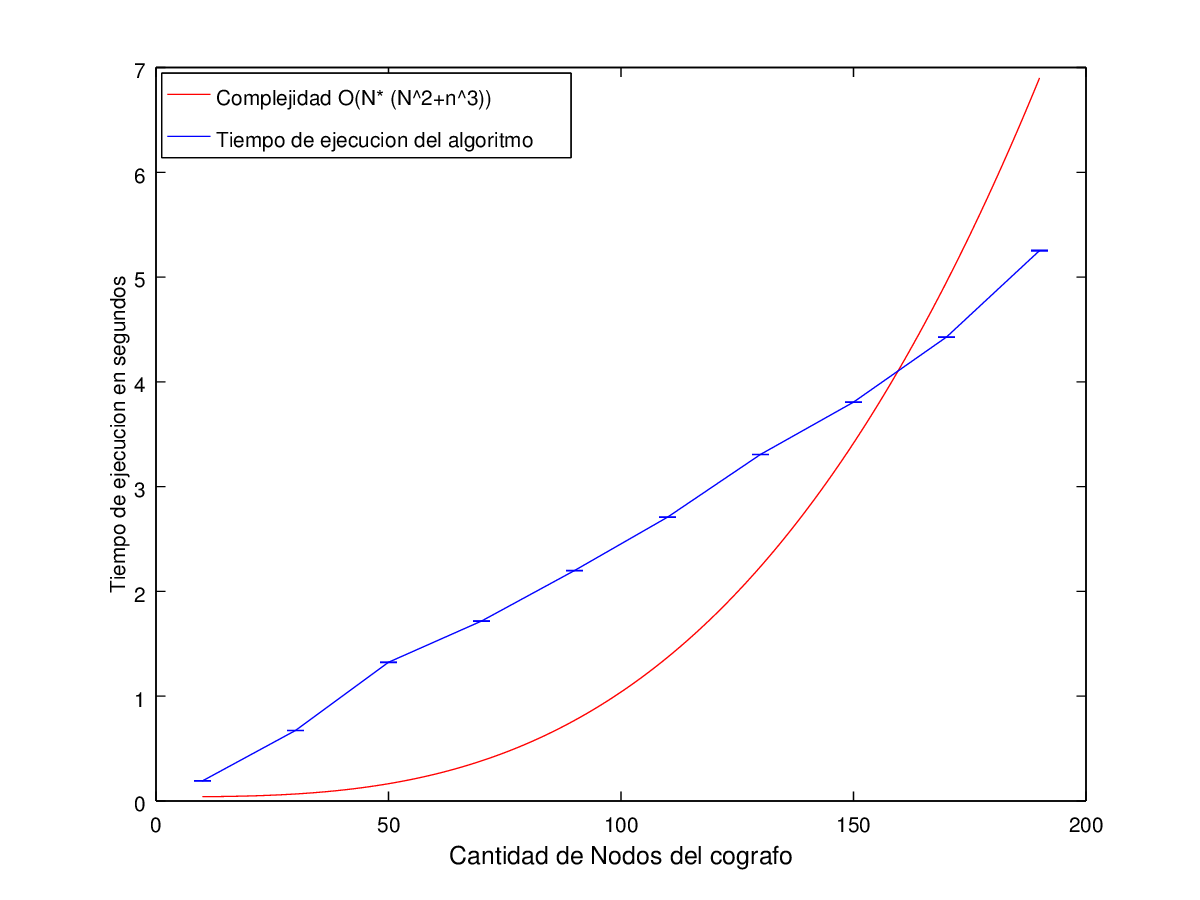
\includegraphics[height=10cm]{graficos/ejercicio3-exp1.png}
       \caption{Experimento 1}
	\end{figure}
        
     	\subsubsection*{Conclusiones}\;
\noindent Se puede observar del gráfico que se respeta la complejidad asintótica propuesta para el algoritmo en caso de hacer variar el $n$ dejando estático el $n$. A pesar de que la curva de tiempo de cómputo esté por encima de la complejidad, a partir de cierto punto, se coloca por debajo de ésta con una curvatura similar o menos pronunciada.
        

\subsubsection*{Experimento 2}\; 

        \noindent Este experimento es similar al anterior pero ahora se variará la cantidad de nodos de cografo ($n_1$) y a la vez también el tamaño (cantidad de nodos) del completo ($n_2$). Lo que trataremos de recrear y observar cual será el comportamiento del tiempo de cómputo a medida que el cografo crece en cantidad de nodos para algún completo arbitrario.

     	\subsubsection*{Datos de entrada}\;
\noindent Los valores de $n_1$ tomados fueron desde $10$ hasta $200$ de $20$ en $20$.\\
       Los valores de $n_2$ son $n_1$/2 para cada $n_1$. \\
        Para generar los grafos de forma aleatoria se utilizó el generador-grafosEspeciales.cpp que se encuentra en la carpeta src y para correrlo se utilizó el exp2.sh que se encuentra en la carpeta exp/ejercicio3/exp2. \\
        Con el fin de acercarse a los valores reales y descartar posibles falsos resultados, se ejecuta la resolución del problema para cada una de los valores de $n_1$ cinco veces considerando luego el promedio entre los valores obtenidos pero graficando también el desvío estándar (la cantidad de repeticiones a realizar fue elegida arbitrariamente).\; 

\subsubsection*{Resultados}\;

            \begin{figure}[H]
      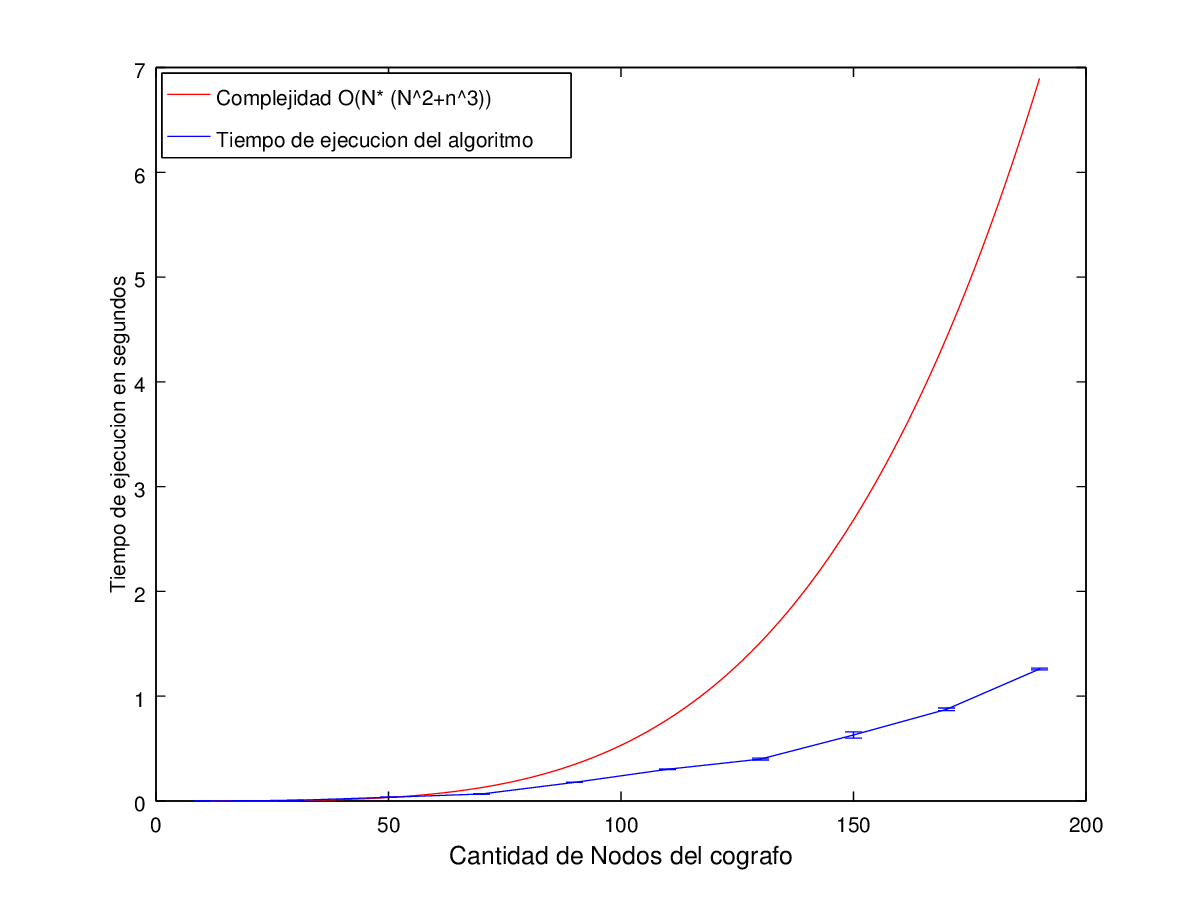
\includegraphics[height=10cm]{graficos/ejercicio3-exp2.png}
       \caption{Experimento 2}
	\end{figure}
        
     	\subsubsection*{Conclusiones}\;
        Se observa que también se respeta la complejidad predicha ya que se ve que la curva del tiempo de ejecución se sitúa por debajo de la curva de complejidad asintótica.\\
        Podemos concluir entonces del experimento que el algoritmo respeta la complejidad propuesta.\\
Pareciera  que la curva de complejidad calculada es de un orden superior al la curva del tiempo de ejecución, esto podría significar, que podría hilarse mas fino en la complejidad propuesta o que quizás el grafo generado al azar y el completo no entrarían dentro del peor caso.









